\documentclass{classes/exam} 
\usepackage{siunitx}
\usepackage{chemfig}
\usepackage{tikz}
\usepackage{physics}
\usepackage{circuitikz}
\usepackage{graphicx}
\graphicspath{ {./images/} }
\usepackage[version=4]{mhchem}
\usepackage{tkz-euclide}
\definecolor{myyellow}{RGB}{254,241,24}
\definecolor{myorange}{RGB}{234,125,1}
\definecolor{fancyorange1}{RGB}{253,138,9}
\definecolor{fancyorange2}{RGB}{246,156,123}
\definecolor{bittersweet}{rgb}{1.0, 0.44, 0.37}
\definecolor{brinkpink}{rgb}{0.98, 0.38, 0.5}
\definecolor{cadetgrey}{rgb}{0.57, 0.64, 0.69}
\definecolor{lightpink}{rgb}{1.0, 0.71, 0.76}
\usepackage{tkz-euclide}
\usetkzobj{all}
\tikzstyle arrowstyle=[scale=1]
\tikzstyle directed=[postaction={decorate,decoration={markings,
		mark=at position .65 with {\arrow[arrowstyle]{stealth}}}}]
\tikzstyle direct=[postaction={decorate,decoration={markings,
		mark=at position .65 with {\arrow[arrowstyle]{stealth reversed}}}}]
\usetikzlibrary{shadings,shapes.geometric,calc, patterns, angles, quotes, arrows.meta, shapes, decorations.pathmorphing, decorations.shapes, decorations.text,calc,angles,quotes,decorations.markings}
\tikzset{>=latex}
\usepackage{chemfig}
\usepackage{multirow}
\usetikzlibrary{quotes,arrows.meta}
%\pagestyle{empty}
\begin{document}
	\begin{flushleft}
		{\kml មន្ទីរអប់រំ យុវជន និងកីឡា រាជធានីភ្នំពេញ\\
			~~~~~~~~~~~~~~~~~សាលាមេតូឌីស្ទកម្ពុជា}
	\end{flushleft}
	\begin{center}
		{\kml ប្រឡងជ្រើសរើសសិស្សពូកែប្រចាំសាលា}\\
			{\kml ផ្នែកអក្សរសិល្ប៍ខ្មែរ គណិតវិទ្យា និងរូបវិទ្យា ថ្នាក់ទី៩ និងថ្នាក់ទី១២}\\
		{\emph{\kob សម័យប្រឡងៈ ថ្ងៃទី៣០ ខែមករា ឆ្នាំ២០២០\\
				វិញ្ញាសាៈ {\kml រូបវិទ្យា ថ្នាក់ទី១២}\\
				រយៈពេលៈ ១៨០នាទី \quad ពិន្ទុៈ ១០០ពិន្ទុ}}
	\end{center}
	{\kml \underline{ប្រធាន}}
	\begin{enumerate}[I]
		\item {\color{magenta}\ks (១០ ពិន្ទុ)} កាំភ្លើងមួយត្រូវបានចាត់ទុកជាម៉ាសុីនកម្តៅ។ គេដឹងថាកាំភ្លើងធ្វើពីដែកដែលមានម៉ាសស្មើ $1.8kg$។ គ្រាប់កាំភ្លើងនេះមានម៉ាស $2.40g$ ហើយពេលបាញ់ចេញមានល្បឿន $320m/s$ និងមានទិន្នផលថាមពលស្មើ $1.10\%$។ សន្មតថាតួ(ដង)កំាភ្លើងស្រូបថាមពលទាំងអស់ដែលបញ្ចេញនិងកើនឡើងសីតុណ្ហភាពស្មើសាច់ក្នុងរយៈពេលខ្លីមុនពេលបាត់បង់ថាមពលកម្តៅខ្លះទៅក្នុងមជ្ឈដ្ឋានបរិយាកាស។\\ គណនាកំណើនសីតុណ្ហភាពនៅក្នុងគ្រាប់កាំភ្លើង។ គេឲ្យកម្តៅម៉ាសដែក $C_{\text{ដែក}}=448J/kg^{\circ}C$។
		\item {\color{magenta}\ks (១០ ពិន្ទុ)} ស៊្វែរបន្ទុកអគ្គិសនីឯកលក្ខណ៍ពីរត្រូវបានគេព្យូរទៅនឹងចំណុចនឹងមួយ ដោយខ្សែមិនយឺតនិងមិនគិតម៉ាសដែលមានប្រវែង $\ell=1.50m$ (ដូចរូប)។ បន្ទុកអគ្គិសនី $q=25.0\mu C$ ត្រូវបានបញ្ជួនទៅឲ្យកូនបាល់នីមួយៗ ក្រោយមកវាច្រានគ្នាចេញបានមុំ $30.0^\circ$ ជាមួយអ័ក្សឈរ។ តើម៉ាសរបស់ស៊្វែនីមួយៗមានតម្លៃប៉ុន្មាន?
		\begin{figure}[H]
			\centering
			\begin{tikzpicture}
			% save length of g-vector and theta to macros
			\pgfmathsetmacro{\Gvec}{1.5}
			\pgfmathsetmacro{\myAngle}{30}
			% calculate lengths of vector components
			\pgfmathsetmacro{\Gcos}{\Gvec*cos(\myAngle)}
			\pgfmathsetmacro{\Gsin}{\Gvec*sin(\myAngle)}
			
			\coordinate (centro) at (0,0);
			\coordinate (y) at (-1.5,-1.0);
			\coordinate (tension) at (-.6,-1.0);
			\node at (1,-1) {$\ell$};
			\node at (-1,-1) {$\ell$};
			\draw[dashed,magenta,-] (centro) -- ++ (0,-1.0) node (mary) [black,below]{$ $};
			\draw[thick] (centro) -- ++(270+\myAngle:3) coordinate (bob);
			\draw[thick] (centro) -- ++(270-\myAngle:3) coordinate (bob);
			\pic [draw, -, "$\theta$", angle eccentricity=1.5] {angle = bob--centro--mary};
			\pic [draw, -, "$\theta$", angle eccentricity=1.5] {angle = tension--bob--y};
			\draw [red, line width=2pt,-stealth] (bob) -- ($(bob)!\Gcos cm!(centro)$) node[ near end, right] {$\overrightarrow{T}$};
			\draw [green!50!black, line width=2pt,-stealth] (bob) -- ($(bob)!\Gsin cm!120:(centro)$)
			coordinate (gsin)
			node[near end, left] {$\overrightarrow{F}_{e}$};
			\draw [blue, line width=2pt,-stealth] (bob) -- ++(0,-\Gvec)
			coordinate (g)
			node[near end,right] {$\overrightarrow{F}_{g}$};
			%\pic [draw, -, "$\theta$", angle eccentricity=1.5] {angle = gcos--bob--g};
			\draw [dashed] (bob) -- (1.5,-2.6) node at (0,-2.6) [black, below] {$d$};
			\draw [dashed] (bob) -- (y);
			\shade [ball color=green!40] (bob) circle[radius=6pt];
			\shade [ball color=green!40] (1.5,-2.6) circle[radius=6pt];
			\fill[pattern = north east lines] ($ (centro) + (-.6,0) $) rectangle ($ (centro) + (.6,0.2) $);
			\draw [line width=2pt] (-.6,0) -- (.6,0);
			\end{tikzpicture}
		\end{figure}
		\item  {\color{magenta}\ks (១០ ពិន្ទុ)} នៅអាកាសយានដ្ឋានមួយ ស្រ្តីម្នាក់កំពុងទាញវ៉ាលីរបស់គាត់ដែលមានម៉ាស $20.0\si{\kilogram}$ ឲ្យផ្លាស់ទីដោយល្បឿនថេរ ហើយប្រើកម្លាំងដែលមានទិសដៅបង្កើតបានមុំ $\theta$ ជាមួយអ័ក្សដេក និងមានតម្លៃ $35.0\si{\newton}$ ដូចបង្ហាញក្នុងរូប។\\ កម្លាំងកកិតដែលមានអំពើលើវ៉ាលីមានតម្លៃស្មើ $20.0\si{\newton}$។
		\begin{enumerate}[k,2]
			\item រកតម្លៃរបស់មុំ $\theta$។
			\item រកតម្លៃរបស់កម្លាំងកែងដែលផ្ទៃដីមានអំពើលើវ៉ាលី។
		\end{enumerate}
		\begin{figure}[H]
			\centering
			\begin{tikzpicture}
			\coordinate (A) at (-.5,-1);
			\coordinate (B) at (.5,0);
			\coordinate (C) at (.5,-1);
			\draw [line width=2pt](A) to (B);
			\draw [dashed](A) to (C);
			\node at (0,0) {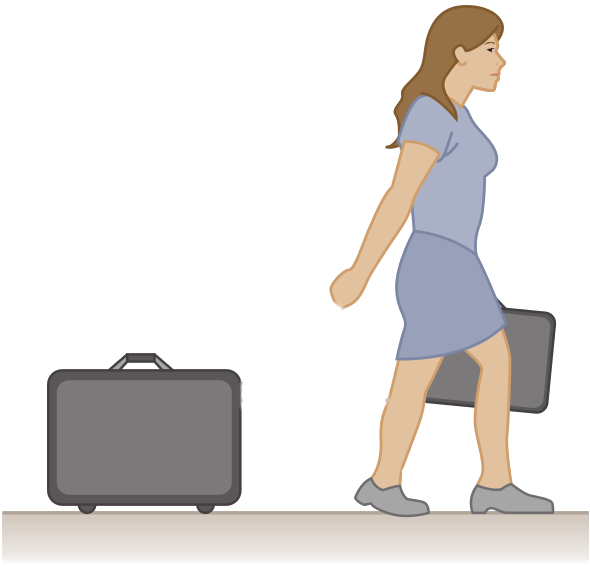
\includegraphics[scale=.24]{woman}};
			\pic [draw, -, "$\theta$", angle eccentricity=1.5, angle radius=.5cm] {angle = C--A--B};
			\end{tikzpicture}
		\end{figure}
		\item {\color{magenta}\ks (១០ ពិន្ទុ)} ផង់នីមួយៗមានម៉ាស $m_{0}$ និងផ្លាស់ទីដោយល្បឿន $v$ តាមបណ្តោយអ័ក្ស $\overrightarrow{ox}$។ គេដឹងថាក្នុងផ្ទៃ $2mm^{2}$ និងក្នុងមួយវិនាទីមានផង់ចំនួន $2\times10^{15}$ ទៅទង្គិចនឹងផ្ទៃនោះ។ គេឲ្យៈ $m_{0}=9.1\times10^{-31}kg$ និង $v=5.0\times10^{15}m/s$។\\
		គេសន្មតថា ទង្គិចរវាងផង់និងផ្ទៃប៉ះជាទង្គិចស្ទក់។
		\begin{enumerate}[k,2]
			\item គណនាកម្លាំងសរុបដែលផង់មានអំពើលើផ្ទៃប៉ះ។
			\item គណនាសម្ពាធសរុបរបស់ផង់លើផ្ទៃប៉ះ។
		\end{enumerate}
		\item {\color{magenta}\ks (១០ ពិន្ទុ)} ប្រសិនបើថាមពលសុីនេទិចគ្រប់គ្រាន់នោះម៉ូលេគុលដែលស្ថិតនៅលើផែនដីអាចរួចផុតពីផែនដីដែលអាចឲ្យវាមានចលនាចាកចេញពីផែនដីជារៀងរហូត។
		\begin{enumerate}[k]
			\item ចូរប្រើប្រាស់ច្បាប់រក្សាថាមពលបង្ហាញថា ថាមពលសុីនេទិចអប្បបរមាដែលត្រូវការដើម្បីឲ្យម៉ូលេគុលអាចខ្ទាតចេញពីផែនដីស្មើនឹង $mgR_{E}$ ដែល $m$ ជាម៉ាសម៉ូលេគុល $g$ ជាសំទុះនៃទម្លាក់សេរីនៅលើផែនដី និង $R_{E}$ ជាកាំរបស់ផែនដី។
			\item គណនាសីតុណ្ហភាពដើម្បីឲ្យថាមពលសុីនេទិចអប្បបរមានេះស្មើនឹងដប់ដងនៃថាមពលសុីនេទិចមធ្យមនៃម៉ូលេគុលអុកសុីសែន។ គេឲ្យៈ $g=9.80m/s^{2},~R_{E}=6.37\times10^{6}m$
		\end{enumerate}
		\item {\color{magenta}\ks (១៥ ពិន្ទុ)} ស៊ីឡាំងក្នុងរូបត្រូវបានបិទដោយពិស្តុងដែលតភ្ជាប់នឹងរ៉ឺស័រមួយមានថេរកម្រាញ $2.00\times 10^{3}\si{\newton/\metre}$។ \\ នៅស្ថានភាពទំនេរនៃរ៉ឺស័រស៊ីឡាំងមានឧស្ម័នចំណុះ $5.00\ell$ ក្រោមសម្ពាធ $1.00\si{atm}$ និងសីតុណ្ហាភាព $20.0^\circ C$។
		\begin{enumerate}[k]
			\item បើពិស្តុងមានមុខកាត់ $0.0100\si{\metre^{2}}$ និងមានម៉ាសអាចចោលបាន។\\ ចូរគណនាកម្ពស់ឡើងដល់របស់ពិស្តុងនៅសីតុណ្ហភាពកើនឡើងដល់ $250^\circ C$។
			\item គណនាសម្ពាធរបស់ឧស្ម័ននៅសីតុណ្ហភាព $250^\circ C$។
		\end{enumerate}
		\begin{figure}[H]
			\centering
			\begin{tikzpicture}[>=Stealth, scale=1.0]
				\node at (0,0) {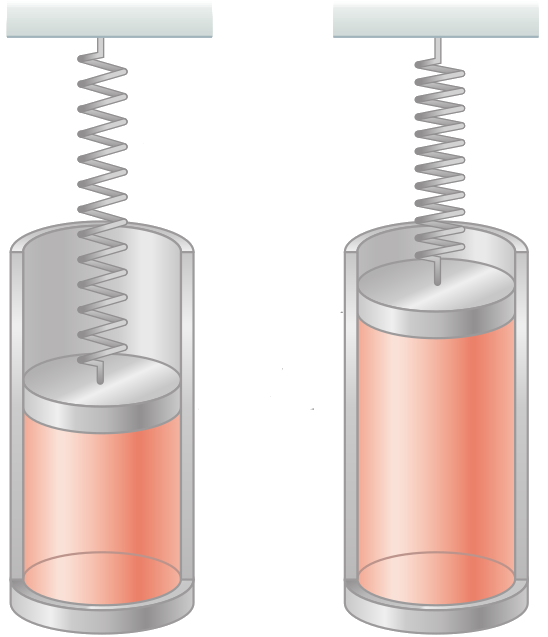
\includegraphics[scale=0.3]{cycinder}};
				\node[right] at (-1.5,2) {$K$};
				\node[below] at (-2,-3.5) {$T=20.0^\circ C$};
				\node[below] at (2,-3.5) {$T=250^\circ C$};
				\draw (-.8,-1) to (.5,-1);
				\draw (.7,0) to (-.5,0);
				\node[left] at (0,-.5) {$h$};
				\draw[<->] (0,-1) to (0,0);
			\end{tikzpicture}
		\end{figure}
		\item {\color{magenta}\ks (១០ ពិន្ទុ)} អង្គធាតុចម្លងរាងស៊ីឡាំងវែងកាំបាត $a$ មួយមានរន្ធប្រហោងរាងស៊ីឡំាងដែលមានអង្កត់ផ្ចិត $a$ តាមបណ្តោយស៊ីឡាំងនេះ(ដូចរូប)។ ចរន្ត $I$ មានទិសដៅចេញក្រៅមកទំព័រ និងមានលក្ខណៈឯកសណ្ឋាន។\\ គណនាដែនម៉ាញេទិច និងទិសដៅរបស់វាជាអនុគមន៍នៃ $\mu_0,~I,~r$ និង $a$ នៅត្រង់៖
		\begin{enumerate}[k,2]
			\item ចំណុច $P_{1}$។
			\item ចំណុច $P_{2}$។
		\end{enumerate}
		\begin{figure}[H]
			\centering
			\begin{tikzpicture}[>=Stealth, scale=1.0]
				\coordinate[label=above:$P_{1}$] (P1) at (0,4);
				\node at (P1) {$\bullet$};
				\coordinate[label=above:$P_{2}$] (P2) at (4,0);
				\node at (P2) {$\bullet$};
				\draw (P1) to (-6,4);
				\draw (P2) to (4,-2.7);
				\draw[<->] (4,-2.7) to (0,-2.7);
				\draw[<->] (-4,0) to (-4,4);
				\draw[color=red!60, fill=red!5] (0,0) circle (2.6cm);
				\draw[color=red!60, fill=white] (0,1.3) circle (1.3cm);
				\draw[color=red!60, fill=white] (0,-1.3) circle (1.3cm);
				\draw[<->] (0,0) to (0,2.6);
				\draw[<->] (0,0) to (0,-2.6);
				\draw[dashed] (-6,0) to (6,0);
				\draw[dashed] (0,2.6) to (0,4);
				\draw[dashed] (0,-2.6) to (0,-3);
				\coordinate[label=right:$a$] (a) at (0,1.3);
				\coordinate[label=right:$a$] (a) at (0,-1.3);
				\coordinate[label=above:$r$] (r) at (2.5,-2.6);
				\coordinate[label=left:$r$] (r) at (-4,2.6);
			\end{tikzpicture}
		\end{figure}
		\item {\color{magenta}\ks (១០ ពិន្ទុ)} គ្រាប់អង្កាំឯកលក្ខណ៍ពីរមានម៉ាស $m$ និងបន្ទុក $q$។ នៅពេលដែលគេដាក់វាក្នុងចានដែលមានផ្នែកខាងក្នុងរាងស៊្វែកាំ $R$ ដោយគ្មានកកិត ហើយជញ្ជាំងរបស់វាមិនចម្លងអគ្គិសនី នោះបន្ទុកទាំងពីរផ្លាស់ទីចេញពីគ្នាដូចបង្ហាញក្នុងរូប។ នៅលក្ខខណ្ឌលំនឹង បន្ទុកស្ថិតនៅចម្ងាយ $R$ ពីគ្នា។ គណនាបន្ទុកអគ្គិសនីរបស់របស់គ្រាប់អង្គាំនីមួយៗ។
		\begin{figure}[H]
			\centering
			\begin{tikzpicture}[>=Stealth, scale=1.0]
				\draw[dashed] (-2,-1) to (0,2);
				\draw[dashed] (2,-1) to (0,2);
				\draw[dashed] (2,-.95) to (-2,-.95);			
				\node at (0,0) {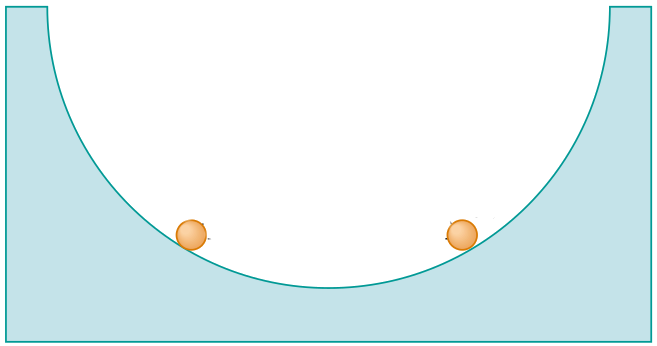
\includegraphics[scale=0.4]{semicircle}};
				\coordinate[label=above right:$m$] (m) at (2,-.8);
				\coordinate[label=above left:$m$] (m) at (-2,-.8);
				\coordinate[label=below:$R$] (R) at (0,-1);
				\coordinate[label=left:$R$] (R) at (-1,.8);
				\coordinate[label=right:$R$] (R) at (1,.8);
			\end{tikzpicture}
		\end{figure}
		\item {\color{magenta}\ks (១៥ ពិន្ទុ)} កូនបាល់មួយដែលមានម៉ូម៉ង់និចល $I=\left(\frac{2}{5}\right)mr^{2}$ រមៀលដោយគ្មានរអិលនៅផ្នែកខាងក្នុងនៃស៊ីឡាំងកាំ $R$ មួយ។ បើស៊ីឡាំងមានចលនារង្វិលជុំវិញអ័ក្សរបស់វា ដោយសំទុះមុំ $\alpha$ តើតម្លៃ $\alpha$ ត្រូវស្មើប៉ុន្មានដើម្បីឲ្យបន្ទាត់ភ្ជាប់រវាងផ្ចិតរបស់បាល់និងផ្ចិតនៃបាតរបស់ស៊ីឡាំងផ្គុំបានមុំ $\theta$ ធៀបនឹងអ័ក្សឈរជានិច្ច?
		\begin{figure}[H]
			\centering
			\begin{tikzpicture}[>=Stealth, scale=1.0]
				\coordinate (O) at (0,0);
				\coordinate (R) at (0,-4);
				\coordinate (R1) at (-1.2,-1.1);
				\coordinate (O1) at (-2,-2);
				\draw[color=red!60, fill=red!5] (0,0) circle (4.0cm);
				\draw[color=red!60, fill=white] (-2,-2) circle (1.15cm);
				\draw[dashed] (0,0) to (0,-4);
				\draw[dashed] (0,0) to (-1.2,-1.1);
				\draw[dashed] (O1) to (-1.5,-3);
				\node[right] at (0,-2) {$R$};
				\node at (-1.6,-2.3) {$r$};
				\node at (O) {$\bullet$};
				\node at (O1) {$\bullet$};
				\pic [draw, -, "$\theta$", angle eccentricity=1.5] {angle = R1--O--R};
				\draw[->] (-4.5,0) arc (0:-20:-5);
				\draw[->] (-3.3,-2) arc (0:-40:-1);
				\node[left] at (-4.5,1) {$\alpha$};
			\end{tikzpicture}
		\end{figure}
	\end{enumerate}
		\begin{flushleft}
			{\kml មន្ទីរអប់រំ យុវជន និងកីឡា រាជធានីភ្នំពេញ\\
				~~~~~~~~~~~~~~~~~សាលាមេតូឌីស្ទកម្ពុជា}
		\end{flushleft}
		\begin{center}
			{\kml ប្រឡងជ្រើសរើសសិស្សពូកែប្រចាំសាលា}\\
			{\kml ផ្នែកអក្សរសិល្ប៍ខ្មែរ គណិតវិទ្យា និងរូបវិទ្យា ថ្នាក់ទី៩ និងថ្នាក់ទី១២}\\
			{\emph{\kob សម័យប្រឡងៈ ថ្ងៃទី៣០ ខែមករា ឆ្នាំ២០២០\\
					វិញ្ញាសាៈ {\kml រូបវិទ្យា ថ្នាក់ទី១២}\\
					រយៈពេលៈ ១៨០នាទី \quad ពិន្ទុៈ ១០០ពិន្ទុ}}
		\end{center}
	{\kml \underline{អត្រាកំណែ}}
	\begin{enumerate}[I]
		\item {\color{magenta}\ks (១០ ពិន្ទុ)} គណនាកំណើនសីតុណ្ហភាពនៅក្នុងគ្រាប់កាំភ្លើង
		\begin{align*}
			\text{យើងមាន}\quad :&\quad W=\Delta K=\frac{1}{2}mv^{2}_{2}-\frac{1}{2}mv^{2}_{1}=\frac{1}{2}mv^{2}_{2}-0\\
			\quad :&\quad W=\frac{1}{2}mv^{2}\\
			\text{ម្យ៉ាងទៀត}\quad:&\quad W=Q_{h}-Q_{c}~\Rightarrow~Q_{c}=Q_{h}-W\\
			\text{តែ}\quad:&\quad e=\frac{W}{Q_{h}}~\Rightarrow~Q_{h}=\frac{W}{e}\\
			\text{យើងបាន}\quad :&\quad Q_{c}=\frac{W}{e}-W=W\left(\frac{1}{e}-1\right)=\frac{1}{2}mv^{2}\left(\frac{1}{e}-1\right)\\
			\text{និង}\quad :&\quad Q_{c}=m'C\Delta T\\
			\quad :&\quad \frac{1}{2}mv^{2}\left(\dfrac{1}{e}-1\right)=m'C\Delta T\\
			\text{នាំឲ្យ}\quad :&\quad \Delta T=\frac{mv^{2}\left(\dfrac{1}{e}-1\right)}{2m'C}\\
			\text{ដោយ}\quad :&\quad m=2.40\si{\gram}=2.40\times 10^{-3}\si{\kilogram},~m'=1.8\si{\kilogram},~v=320\si{\metre/\second}\\
			\quad :&\quad C_{\text{ដែក}}=448\si{\joule/\kilogram\celsius},~e=1.10\%=0.011\\
			\text{យើងបាន}\quad :&\quad \Delta T=\frac{2.40\times 10^{-3}\left(320\right)^{2}\left(\dfrac{1}{0.011}-1\right)}{2\times 1.8 \times 448}=13.7\si{\celsius}\\
			\text{ដូចនេះ}\quad :&\quad \Delta T=13.7\si{\celsius}
		\end{align*}
		\item {\color{magenta}\ks (១០ ពិន្ទុ)} ម៉ាសរបស់ស៊្វែនីមួយៗ
		\begin{figure}[H]
			\centering
			\begin{tikzpicture}
				\pgfmathsetmacro{\Gvec}{1.5}
				\pgfmathsetmacro{\myAngle}{30}
				\pgfmathsetmacro{\Gcos}{\Gvec*cos(\myAngle)}
				\pgfmathsetmacro{\Gsin}{\Gvec*sin(\myAngle)}
				\coordinate (centro) at (0,0);
				\coordinate (y) at (-1.5,-1.0);
				\coordinate (tension) at (-.6,-1.0);
				\node at (1,-1) {$\ell$};
				\node at (-1,-1) {$\ell$};
				\draw[green!50!black, line width=2pt,-stealth, ->] (-1.5,-2.6) to (-.6,-2.6) node [below] (-.6,-2.6) {$\overrightarrow{T}_{x}$};
				\draw[blue, line width=2pt,-stealth, ->] (-1.5,-2.5) to (-1.5,-1.4) node [left] (-1.5,-1.4) {$\overrightarrow{T}_{y}$};
				\draw[red, line width=2pt,-stealth, ->] (-1.5,-2.6)  to (-2.2, -3.8) node[below] (-2.2, -3.8) {$\overrightarrow{R}$};
				\draw[dashed,magenta,-] (centro) -- ++ (0,-2.6) node (mary) [black,below]{$ $};
				\draw[thick] (centro) -- ++(270+\myAngle:3) coordinate (bob);
				\draw[thick] (centro) -- ++(270-\myAngle:3) coordinate (bob);
				\pic [draw, -, "$\theta$", angle eccentricity=1.5] {angle = bob--centro--mary};
				\pic [draw, -, "$\theta$", angle eccentricity=1.5] {angle = tension--bob--y};
				\draw [red, line width=2pt,-stealth] (bob) -- ($(bob)!\Gcos cm!(centro)$) node[ near end, right] {$\overrightarrow{T}$};
				\draw [green!50!black, line width=2pt,-stealth] (bob) -- ($(bob)!\Gsin cm!120:(centro)$)
				coordinate (gsin)
				node[near end, left] {$\overrightarrow{F}_{e}$};
				\draw [blue, line width=2pt,-stealth] (-1.5,-2.6) to (-1.5,-3.8) node[right] (-1.5,-4) {$\overrightarrow{F}_{g}$};
				\draw [dashed] (bob) -- (1.5,-2.6) node at (0,-2.6) [black, below] {$d$};
				\draw [dashed] (bob) -- (y);
				\shade [ball color=green!40] (bob) circle[radius=6pt];
				\shade [ball color=green!40] (1.5,-2.6) circle[radius=6pt];
				\fill[pattern = north east lines] ($ (centro) + (-.6,0) $) rectangle ($ (centro) + (.6,0.2) $);
				\draw [line width=2pt] (-.6,0) -- (.6,0);
				\draw[dashed] (-1.5,-1.5)  to (-.9, -1.5);
				\draw[dashed] (-.9,-1.5)  to (-.9, -2.6);
				\draw[dashed] (-2.2,-3.8)  to (-1.5, -3.8);
				\draw[dashed] (-2.2,-2.6)  to (-2.2, -3.8);
			\end{tikzpicture}
		\end{figure}
		\begin{align*}
			\text{លក្ខណ្ឌលំនឹង ឬគោលការណ៍និចលភាព}\quad :&\quad \Sigma \overrightarrow{F}=\vec{0}\\
			\text{ឬ}\quad :&\quad \overrightarrow{F}{e}+\overrightarrow{T}_{x}+\overrightarrow{T}_{y}+\overrightarrow{F}_{g}+\overrightarrow{T}+\overrightarrow{R}=\vec{0}\\
			\text{ដែល}\quad :&\quad \overrightarrow{F}_{e}+\overrightarrow{T}_{x}=\vec{0}~\text{នោះ}~F_{e}=T_{x}\\
			\text{តែ}\quad:&\quad F_{e}=k_{e}\frac{q^{2}}{d^{2}}~\text{និង}~T_{x}=T\sin\theta\\
			\quad :&\quad \sin\theta=\frac{\dfrac{d}{2}}{\ell}~\Rightarrow d=2\ell\sin 30^\circ=2\ell\cdot\frac{1}{2}=\ell\\
			\text{គេបាន}\quad :&\quad T\sin\theta = k_{e}\frac{q^{2}}{\ell^{2}}\quad\left(1\right)\\
			\text{ម្យ៉ាងទៀត}\quad :&\quad \overrightarrow{T}_{y}+\overrightarrow{F}_{g}=\vec{0}~\text{ឬ}~T_{y}=F_{g}\\
			\text{ដែល}\quad :&\quad T_{y}=T\cos\theta~\text{និង}~F_{g}=mg\\
			\quad :&\quad T\cos\theta = mg~\Rightarrow~T=\frac{mg}{\cos\theta}\quad \left(2\right)\\
			\text{តាម $\left(1\right)$ និង $\left(2\right)$ គេបាន}\quad :&\quad mg\frac{\sin\theta}{\cos\theta}=k_{e}\frac{q^{2}}{\ell^{2}}~\Rightarrow~m=\frac{k_{e}}{g\tan\theta}\left(\frac{q}{\ell}\right)^{2}\\
			\text{ដោយ}\quad :&\quad k_{e}=9\times 10^{9}\si{SI},~g=9.80\si{\metre/\second^{2}},~q=25.0\mu C=25\times 10^{-6} C\\
			\quad :&\quad \ell=1.5m,~\theta=30.0^\circ~\Rightarrow~\tan 30^\circ=\frac{1}{\sqrt{3}}\\
			\text{ដូចនេះ}\quad :&\quad m=\frac{k_{e}\sqrt{3}}{g}\left(\frac{q}{\ell}\right)^{2}~\left(\si{\kilogram}\right)
		\end{align*}
		\item  {\color{magenta}\ks (១០ ពិន្ទុ)}
		\begin{figure}[H]
			\centering
			\begin{tikzpicture}
			\coordinate (A) at (-.5,-1);
			\coordinate (B) at (.5,0);
			\coordinate (C) at (.5,-1);
			\coordinate (D) at (-.5,0);
			\draw [line width=2pt](A) to (B);
			\draw [dashed](A) to (C);
			\draw[blue, line width=2pt,-stealth] (A) to (C);
			\node[below] at (.4,-1) {$\overrightarrow{F}_{x}$}; 
			\draw[blue, line width=2pt,-stealth] (A) to (D);
			\node[above] at (D) {$\overrightarrow{F}_{y}$};
			\draw[dashed] (D) to (B) to (C);
			\node at (0,0) {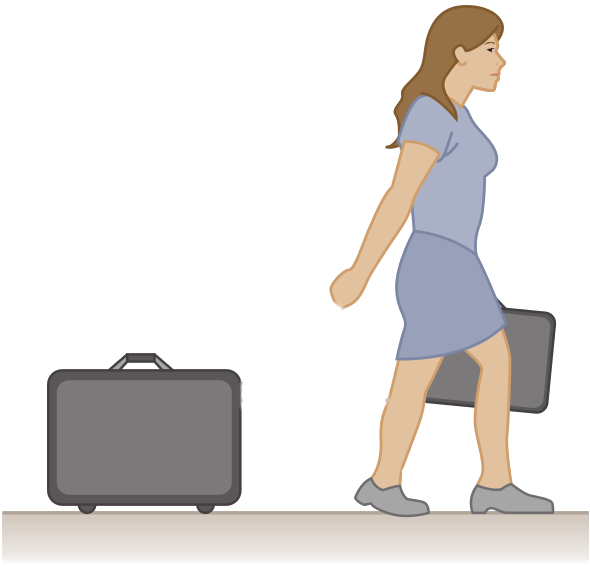
\includegraphics[scale=.24]{woman}};
			\pic [draw, -, "$\theta$", angle eccentricity=1.5, angle radius=.5cm] {angle = C--A--B};
			\draw[blue, line width=2pt,-stealth] (-1.3,-1.3) to (-1.3,-3) node[right] (-1.3,-3) {$\overrightarrow{w}=m\vec{g}$};
			\draw[blue, line width=2pt,-stealth] (-1.2,-1.95) to (-1.2,0) node[above] (-1.2,0) {$\overrightarrow{F}_{N}$};
			\draw[blue, line width=2pt,-stealth] (-1.2,-1.9) to (-3,-1.9) node[left] (-3,-1.9) {$\overrightarrow{f}_{k}$};
		\end{tikzpicture}
		\end{figure}
		\begin{enumerate}[k]
			\item រកតម្លៃរបស់មុំ $\theta$
			\begin{align*}
				\text{លក្ខណ្ឌលំនឹង}\quad :&\quad \Sigma \overrightarrow{F}=\vec{0}\\
				\text{ឬ}\quad :&\quad \overrightarrow{F}_{N}+\overrightarrow{w}+\overrightarrow{f}_{k}+\overrightarrow{F}_{x}+\overrightarrow{F}_{y}=\vec{0}\\
				\text{តាម $\left(ox\right)$}\quad :&\quad \overrightarrow{f}_{k}+\overrightarrow{F}_{x}=\vec{0}~\text{នោះ}\quad F_{x}=f_{k}\\
				\quad :&\quad F\cos\theta=f_{k}~\Rightarrow~\cos\theta=\frac{f_{k}}{F}
			\end{align*}
			\begin{align*}
				\text{ដោយ}\quad :&\quad f_{k}=20.0\si{\newton},~F=35.0\si{\newton}\\
				\text{នាំឲ្យ}\quad :&\quad \cos\theta=\frac{20}{35}=0.571\\
				\text{ដូចនេះ}\quad :&\quad \theta =55.2^\circ
			\end{align*}
			\item រកតម្លៃរបស់កម្លាំងកែងដែលផ្ទៃដីមានអំពើលើវ៉ាលី
			\begin{align*}
				\text{យើងមាន}\quad :&\quad \overrightarrow{F}_{N}+\overrightarrow{w}+\overrightarrow{F}_{y}=\vec{0}~\text{ឬ}~F_{N}-W+F_{y}=0\\
				\quad :&\quad F_{N}=W-F_{y}=mg-F\sin\theta\\
				\text{ដោយ}\quad :&\quad m=20.0\si{\kilogram},~g=9.80\si{\metre/\second^{2}},~F=35.0\si{\newton},~\theta =55.2^\circ\\
				\text{គេបាន}\quad :&\quad F_N=20\times 9.80-35\left(0.821\right)=167\si{\newton}\\
				\text{ដូចនេះ}\quad :&\quad F_{N}=167\si{\newton}
			\end{align*}
		\end{enumerate}
		\item {\color{magenta}\ks (១០ ពិន្ទុ)}
		\begin{enumerate}[k]
			\item គណនាកម្លាំងសរុបដែលផង់មានអំពើលើផ្ទៃប៉ះ
			\begin{align*}
				\text{យើងមាន}\quad :&\quad F\cdot\Delta t=m\Delta v=N\cdot m_{0}\cdot v~\left(\text{ទង្គិចស្ទក់}~\Delta v=v\right)\\
				\text{នាំឲ្យ}\quad :&\quad F=\frac{N\cdot m_{0}\cdot v}{\Delta t}\\
				\text{ដោយ}\quad :&\quad N=2\times 10^{15},~m_{0}=9.1\times 10^{-31}\si{\kilogram},~v=5.0\times 10^{15}\si{\metre/\second},~\Delta t=1.0s\\
				\text{យើងបាន}\quad :&\quad F=\frac{2\times 10^{15}\times 9.1\times 10^{-31}\times 5\times 10^{15}}{1}=9.1\si{\newton}\\
				\text{ដូចនេះ}\quad :&\quad F=9.1\si{\newton}
			\end{align*}
			\item គណនាសម្ពាធសរុបរបស់ផង់លើផ្ទៃប៉ះ
			\begin{align*}
				\text{តាម}\quad :&\quad P=\frac{F}{A}\\
				\text{ដោយ}\quad :&\quad F=9.1\si{\newton},~A=2\si{\milli \metre^{2}}=2\times 10^{-4}\si{\metre^{2}}\\
				\text{គេបាន}\quad :&\quad P=\frac{9.1}{2\times 10^{-4}}=4.55\times 10^{4}\si{\pascal}\\
				\text{ដូចនេះ}\quad :&\quad P=4.55\times 10^{4}\si{\pascal}
			\end{align*}
		\end{enumerate}
			\item {\color{magenta}\ks (១០ ពិន្ទុ)}
		\begin{enumerate}[k]
			\item ចូរបង្ហាញថា ថាមពលសុីនេទិចអប្បបរមាដែលត្រូវការដើម្បីឲ្យម៉ូលេគុលអាចខ្ទាតចេញពីផែនដីស្មើនឹង $mgR_{E}$ ដែល $m$ ជាម៉ាសម៉ូលេគុល $g$ ជាសំទុះនៃទម្លាក់សេរីនៅលើផែនដី និង $R_{E}$ ជាកាំរបស់ផែនដី
			\begin{align*}
				\text{តាមច្បាប់រក្សាថាមពល}\quad :&\quad \Delta K=\Delta U~\Leftrightarrow ~ K=U~\text{ឬ}~K=mgh\\
				\text{ដោយ}\quad :& \quad h=R_{E}\\
				\text{ដូចនេះ}\quad :&\quad K_{min}=mgR_{E}\quad \text{ពិត}
			\end{align*}
			\newpage
			\item គណនាសីតុណ្ហភាពដើម្បីឲ្យថាមពលសុីនេទិចអប្បបរមានេះស្មើនឹងដប់ដងនៃថាមពលសុីនេទិចមធ្យមនៃម៉ូលេគុលអុកសុីសែន
			\begin{align*}
				\text{ដោយ}\quad :&\quad K_{min}=10\left(K_{av}\right)~\Leftrightarrow ~ K_{min}=10\left(\frac{3}{2}k_{B}T\right)=15k_{B}T\\
				\quad :&\quad T=\frac{K_{min}}{15k_{B}}=\frac{mgR_{E}}{15k_{B}}~\text{តែ}~m=\frac{M}{N_{A}}\\
				\text{នាំឲ្យ}\quad :&\quad T=\frac{MgR_{E}}{15k_{B}N_{A}}=\frac{MgR_{E}}{15R}\\
				\text{ដោយ}\quad :& \quad R_{E}=6.37\times 10^{6}m,~R=8.31\si{\joule/\mole\cdot\kelvin},~g=9.80\si{\metre/\second^{2}},~M=32.0\si{\gram}=32\times 10^{-3}\si{\kilogram}\\
				\text{គេបាន}\quad :&\quad T=\frac{32\times 10^{-3}\times 9.80\times 6.37\times 10^{6}}{15\times 8.31}=1.60\times 10^{4}\si{\kelvin}\\
				\text{ដូចនេះ}\quad :&\quad T=1.60\times 10^{4}\si{\kelvin}
			\end{align*}
		\end{enumerate}
		\item {\color{magenta}\ks (១៥ ពិន្ទុ)}
		\begin{enumerate}[k]
			\item ចូរគណនាកម្ពស់ឡើងដល់របស់ពិស្តុងនៅសីតុណ្ហភាពកើនឡើងដល់ $250^\circ C$
			\begin{align*}
				\text{តាម}\quad :&\quad \frac{P_{1}V_{1}}{T_{1}}=\frac{P_{2}V_{2}}{T_{2}}\\
				\text{ដោយ}​\quad :&\quad V_{2}=V_{1}+Ah~\text{និង}~P_{2}=P_{1}+\frac{F}{A}=P_{1}+\frac{kh}{A}\\
				\text{យើងបាន}\quad :&\quad \frac{P_{1}V_{1}}{T_{1}}=\frac{\left(P_{1}+\dfrac{kh}{A}\right)\left(V_{1}+Ah\right)}{T_{2}}~\text{ឬ}~ \frac{P_{1}V_{1}}{T_{1}}T_{2}=\left(P_{1}+\frac{kh}{A}\right)\left(V_{1}+Ah\right)\\
				\text{ដោយ}\quad :&\quad k=2\times 10^{3}\si{\newton/\metre},~P_{1}=1\si{atm}=1.013\times 10^{5}\si{\pascal},~V_{1}=5.00\si{\litre}=5\times 10^{-3}\si{\metre^{3}},~A=0.01\si{\metre^{2}}\\
				\quad :&\quad T_{1}=20.0\si{\celsius}=293\si{\kelvin},~T_{2}=250\si{\celsius}=523\si{\kelvin}\\
				\text{យើងបាន}\quad :&\quad \frac{1.013\times 10^{5}\times 5\times 10^{-3}\times 523}{293}=\left(1.013\times 10^{5}+\dfrac{2\times 10^{3}h}{0.01}\right)\left(5\times 10^{-3}+0.01h\right)\\
				\quad :&\quad 2000h^{2}+2013h-397=0\\
				\text{តាម}\quad :&\quad \Delta = \left(2013\right)^{2}-4\left(2000\right)\left(-397\right)=273\times 10^{4}\\
				\text{នោះ}\quad :&\quad \sqrt{\Delta}=\sqrt{273\times 10^{4}}=\pm 2689\\
				\text{ដែល}\quad:&\quad h=\frac{-2013-2689}{2\times 2000}=-1.175<0\quad\left(\text{មិនយក}\right)\\
				\quad :&\quad h=\frac{-2013+2689}{2\times 2000}=0.169>0\quad\left(\text{យក}\right)\\
				\text{ដូចនេះ}\quad :&\quad h=0.169\si{\metre}
			\end{align*}
			\item គណនាសម្ពាធរបស់ឧស្ម័ននៅសីតុណ្ហភាព $250^\circ C$
			\begin{align*}
				\text{យើងមាន}\quad :&\quad P_{2}=P_{1}+\frac{kh}{A}\\
				\text{ដោយ}\quad :&\quad k=2\times 10^{3}\si{\newton/\metre},~P_{1}=1\si{atm}=1.013\times 10^{5}\si{\pascal},~A=0.01\si{\metre^{2}},~h=0.169\si{\metre}\\
				\text{យើងបាន}\quad :&\quad P_{2}=1.013\times 10^{5}+\frac{2\times 10^{3}\times 0.169}{0.01}=1.35\times 10^{5}\si{\pascal}\\
				\text{ដូចនេះ}\quad :&\quad P_{2}=1.35\times 10^{5}\si{\pascal}
			\end{align*}
		\end{enumerate}
		\item {\color{magenta}\ks (១០ ពិន្ទុ)} គណនាដែនម៉ាញេទិច និងទិសដៅរបស់វាជាអនុគមន៍នៃ $\mu_0,~I,~r$ និង $a$ នៅត្រង់៖
		\begin{figure}[H]
			\centering
			\begin{tikzpicture}[>=Stealth, scale=1.0]
			\coordinate[label=above:$P_{1}$] (P1) at (0,4);
			\coordinate (B1) at (3.4,-1.5);
			\coordinate (B2) at (4.6,-1.5);
			\coordinate (O) at (0,0);
			\coordinate (O1) at (0,1.3);
			\coordinate (O2) at (0,-1.3);
			\coordinate (M) at (4,-1.5);
			\coordinate (I1) at (0,.8);
			\coordinate (I2) at (0,-.8);
			\node at (P1) {$\bullet$};
			\coordinate[label=right:$P_{2}$] (P2) at (4,0);
			\node at (P2) {$\bullet$};
			\draw [->](P1) to (-2,4) node[below] (-2,4) {$\overrightarrow{B}_{s}$};
			\pic [draw, -, "$\theta$", angle eccentricity=1.6, angle radius=.5cm] {angle = B1--P2--M};
			\pic [draw, -, "$\theta$", angle eccentricity=1.6, angle radius=.5cm] {angle = M--P2--B2};
			\draw[->] (0,4.1) to (1.5,4.1) node[above] (1.5,4.1) {$-\overrightarrow{B}_{1}$};
			\draw[->] (0,3.93) to (1,3.93) node[below] (1,3.93) {$-\overrightarrow{B}_{2}$};
			\draw[color=red!60,fill=red!5] (0,0) circle (2.6cm);
			\draw[color=red!60, fill=white] (0,1.3) circle (1.3cm);
			\draw[color=red!60, fill=white] (0,-1.3) circle (1.3cm);
			\draw[->] (P2) to (B1) node[left] (B1) {$-\overrightarrow{B}'_{1}$};
			\draw[->] (P2) to (B2) node[right] (B2) {$-\overrightarrow{B}'_{2}$};
			\draw[->] (P2) to (4,2) node[right] (4,2) {$\overrightarrow{B}_{s}$};
			\draw[dashed] (P2) to (M);
			\coordinate[label=left:{$\frac{a}{2}$}] (a) at (I1);
			\coordinate[label=left:{$\frac{a}{2}$}] (a) at (I2);
			\draw[dashed, line width=1pt] (P1) to (O2);
			\draw[dashed, line width=1pt] (P2) to (O1);
			\draw[dashed, line width=1pt] (P2) to (O2);
			\draw[dashed, line width=1pt] (P2) to (O);
			\pic [draw, -, "$\theta$", angle eccentricity=1.6, angle radius=1cm] {angle = I1--P2--O};
			\node[below] at (1.5,0) {$r$};
			\node[left] at (0,3) {$r$};
			\draw[red, ->, line width=2pt] (1.5,.8) to (2.5,2.2) node[above] (2,2.2) {$\sqrt{r^{2}+\left(\dfrac{a}{2}\right)^{2}}$};
			\end{tikzpicture}
		\end{figure}
		\begin{enumerate}[k]
			\item ចំណុច $P_{1}$
			\begin{center}
				ចរន្តអគ្គិសនី $I$ ត្រូវមាននៅក្នុងអង្គធាតុចម្លងនូវដង់ស៊ីតេចរន្ត $J=\frac{I}{A}$\\
				ដែលក្នុងរកណីនេះគេអាចរក $A$
			\end{center}
			\begin{align*}
				\text{ដោយ}\quad :&\quad A=\pi\left[a^{2}-\frac{a^{2}}{4}-\frac{a^{2}}{4}\right]=\frac{\pi a^{2}}{2}\\
				\text{គេបាន}\quad :&\quad J=\frac{2I}{\pi a^{2}}\\
				\text{យើងមាន}\quad :&\quad B_{s}=\frac{\mu_{0}J\left(\pi a^{2}\right)}{2\pi r} ,~B_{1}=\frac{\mu_{0}J\pi\left(\dfrac{a}{2}\right)^{2}}{2\pi\left(r-\dfrac{a}{2}\right)},~
				B_{2}=\frac{\mu_{0}J\pi\left(\dfrac{a}{2}\right)^{2}}{2\pi\left(r+\dfrac{a}{2}\right)}\\
				\quad :&\quad B=B_{s}-B_{1}-B_{2}=\frac{\mu_{0}J\pi a^{2}}{2\pi}\left[\frac{1}{r}-\frac{1}{4\left(r-\dfrac{a}{2}\right)}-\frac{1}{4\left(1+\dfrac{a}{2}\right)}\right]\\
				\text{នាំឲ្យ}\quad:&\quad B=\frac{\mu_{0}\left(2I\right)}{2\pi}\left[\frac{4r^{2}-a^{2}-2r^{2}}{4r\left(r^{2}-\dfrac{a^{2}}{4}\right)}\right]=\frac{\mu_{0}I}{\pi r}\left(\frac{2r^{2}-a^{2}}{4r^{2}-a^{2}}\right)\\
				\text{ដូចនេះ}\quad :&\quad B= \frac{\mu_{0}I}{\pi r}\left(\frac{2r^{2}-a^{2}}{4r^{2}-a^{2}}\right)\quad \text{វាមានទិសដៅឆ្ពោះទៅខាងឆ្វេង។}
			\end{align*}
			\item ចំណុច $P_{2}$
			\begin{align*}
				\text{នៅត្រង់ $P_{2}$ គេបាន៖}\quad :&\quad B_{s}=\frac{\mu_{0}J\left(\pi a^{2}\right)}{2\pi r}\\
				\text{និង}\quad :&\quad B'_{1}=B'_{2}=\frac{\mu_{0}J\pi\left(\dfrac{a}{2}\right)^{2}}{2\pi\sqrt{r^{2}+\left(\dfrac{a}{2}\right)^{2}}}
			\end{align*}
			\begin{center}
				តាមរូបខាងលើ យើងឃើញថាកុំប៉ូសង់តាមបន្ទាត់ដេកនៃ $B'_{1}$ និង $B'_{2}$ ទប់ទល់គ្នា។ ចំពោះកុំប៉ូសង់តាមបន្ទាត់ឈរគេអាចសរសេរដូចតទៅ៖
			\end{center}
			\begin{align*}
				\quad:&\quad B=B_{s}-B'_{1}\cos\theta-B'_{2}\cos\theta=\frac{\mu_{0}J\left(\pi a^{2}\right)}{2\pi r}-2\left(\frac{\dfrac{\mu_{0} J\pi a^{2}}{4}}{2\pi\sqrt{r^{2}+\dfrac{a^{2}}{4}}}\right)\frac{r}{\sqrt{r^{2}+\dfrac{a^{2}}{4}}}\\
				\quad :&\quad B=\frac{\mu_{0}\left(2I\right)}{2\pi r}\left[1-\frac{2r^{2}}{4r^{2}+a^{2}}\right]\\
				\text{ដូចនេះ}\quad :&\quad B=\frac{\mu_{0} I}{\pi r}\left(\frac{2r^{2}+a^{2}}{4r^{2}+a^{2}}\right)\quad \text{វាមានទិសដៅឆ្ពោះទៅខាងលើ(មកទំព័រ)។}
			\end{align*}
		\end{enumerate}
		\item {\color{magenta}\ks (១៥ ពិន្ទុ)}
		គណនាបន្ទុកអគ្គិសនីរបស់របស់គ្រាប់អង្គាំនីមួយៗ
		\begin{figure}[H]
			\centering
			\begin{tikzpicture}[>=Stealth, scale=1.0]
			\draw[dashed] (-2,-1) to (0,2);
			\draw[dashed] (2,-1) to (0,2);
			\draw[dashed] (2,-.95) to (-2,-.95);	
			\coordinate (A) at (-1.9,-.9);	
			\coordinate (B) at (-1.3,0);
			\coordinate (C) at (2,-.95);
			\node at (0,0) {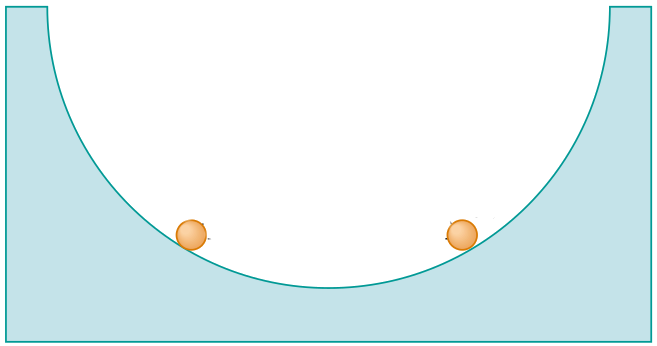
\includegraphics[scale=0.4]{semicircle}};
%			\coordinate[label=above right:$m$] (m) at (2,-.8);
%			\coordinate[label=above left:$m$] (m) at (-2,-.8);
			\coordinate[label=below:$R$] (R) at (0,-1);
			\coordinate[label=left:$R$] (R) at (-1,.8);
			\coordinate[label=right:$R$] (R) at (1,.8);
			\draw[blue, line width=2pt,-stealth] (A) to (-1.9,-2) node[below] at (-1.9,-2) {$\overrightarrow{w}$};
			\draw[blue, line width=2pt,-stealth] (A) to (-2.7,-.9) node[left] at (-2.7,-.9) {$\overrightarrow{F}_{e}$};
			\draw[blue, line width=2pt,-stealth] (A) to (B);
			\node[left] at (-1.3,.2) {$\overrightarrow{F}_{N}$};
			\pic [draw, -, "$60^\circ$", angle eccentricity=1.6, angle radius=.5cm] {angle = C--A--B};
			\end{tikzpicture}
		\end{figure}
		\begin{center}
			ចានមានអំពើលើគ្រាប់អង្កាំនីមួយៗដោយកម្លាំង $\overrightarrow{F}_{N}$ ដែលមានទិសផ្គុំបាន $60.0^\circ$ ធៀបនឹងអ័ក្សដេក។\\
			ដោយប្រើរូបខាងក្រោម គេបានៈ
		\end{center}
		\begin{align*}
			\text{លក្ខខណ្ឌលំនឹង}\quad :&\quad \overrightarrow{F}_{e}+\overrightarrow{w}+\overrightarrow{F}_{N}=\vec{0}\\
			\text{ម្យ៉ាងទៀត}\quad :&\quad \overrightarrow{F}_{e}+\overrightarrow{w}+\overrightarrow{F}_{N}\cos 60.0^\circ+\overrightarrow{F}_{N}\sin 60.0^\circ=\vec{0}\\
			\text{តាម $\left(ox\right)$}\quad :&\quad F_{e}-F_{N}\cos 60.0^\circ=0~\text{ឬ}~F_{e}=F_{N}\cos 60.0^\circ\quad\left(1\right)\\
			\text{តាម $\left(oy\right)$}\quad :&\quad F_{N}\sin 60.0^\circ-mg=0~\text{ឬ}~F_N\sin 60.0^\circ=mg\\
			\text{នោះ}\quad :&\quad F_{N}=\frac{mg}{\sin 60.0^\circ}\quad\left(2\right)\\
			\text{តាម $\left(1\right)$ និង $\left(2\right)$}\\
			\text{យើងបាន}\quad :&\quad k_{e}\frac{q^{2}}{R^{2}}=\frac{mg}{\tan 60.0^\circ}=\frac{mg}{\sqrt{3}}\\
			\text{ដូចនេះ}\quad :&\quad q=R\left(\frac{mg}{k_{e}\sqrt{3}}\right)^{\frac{1}{2}}
		\end{align*}
		\newpage
		\item {\color{magenta}\ks (១៥ ពិន្ទុ)} តើតម្លៃ $\alpha$ ត្រូវស្មើប៉ុន្មានដើម្បីឲ្យបន្ទាត់ភ្ជាប់រវាងផ្ចិតរបស់បាល់និងផ្ចិតនៃបាតរបស់ស៊ីឡាំងផ្គុំបានមុំ $\theta$ ធៀបនឹងអ័ក្សឈរជានិច្ច?
		\begin{figure}[H]
			\centering
			\begin{tikzpicture}[>=Stealth, scale=1.0]
			\coordinate (O) at (0,0);
			\coordinate (R) at (0,-4);
			\coordinate (R1) at (-1.2,-1.1);
			\coordinate (O1) at (-2,-2);
			\draw[color=red!60, fill=red!5] (0,0) circle (4.0cm);
			\draw[color=red!60, fill=white] (-2,-2) circle (1.15cm);
			\draw[dashed] (0,0) to (0,-4);
			\draw[dashed] (0,0) to (-1.2,-1.1);
			\draw[dashed] (O1) to (-1.5,-3);
			\node[right] at (0,-2) {$R$};
			\node at (-1.6,-2.3) {$r$};
			\node at (O) {$\bullet$};
			\node at (O1) {$\bullet$};
			\pic [draw, -, "$\theta$", angle eccentricity=1.5] {angle = R1--O--R};
			\draw[->] (-4.5,0) arc (0:-20:-5);
			\draw[->] (-3.3,-2) arc (0:-40:-1);
			\node[left] at (-4.5,1) {$\alpha$};
			\end{tikzpicture}
		\end{figure}
		\begin{center}
			តាងកម្លាំងកកិតលើផ្ទៃរបស់បាល់គឺ $F$។ កម្លាំង $F$ ត្រូវទប់ទល់នឹងកំប៉ូសង់នៃទម្ងន់ដែលមានទិសតាមតង់សង់
		\end{center}
		\begin{align*}
			\text{ម៉ូម៉ង់កម្លាំងបង្វិលទៅលើបាល់គឺ}\quad :&\quad \tau=Fr\\
			\text{គេសរសេរអាំងតង់ស៊ីតេរបស់កម្លាំង $F$ ដោយប្រើប្រាស់កន្សោម}\quad :&\quad F=mg\sin\theta\\
			\text{គេបាន}\quad :&\quad \tau=mgr\sin\theta\\
			\text{ម៉្យាងទៀត ម៉ូម៉ង់កម្លាំងបង្វិលនេះគឺ}\quad :&\quad \tau =I\alpha_{b}\\
			\text{ដែល $\alpha_{b}$ នេះគឺសំទុះមុំនៃចលនាបាល់ ហើយជាប់ទាក់ទង់នឹង $\alpha$ នៃស៊ីឡាំងតាមកន្សោម}\quad :&\quad \alpha_{b}=\left(\frac{R}{r}\right)\alpha
		\end{align*}
		\begin{align*}
			\text{ដោយប្រើកន្សោម $\tau=I\alpha_{b}$ គេបាន}\quad :&\quad mgr\sin\theta=\left(\frac{2}{5}mr^{2}\right)\left(\frac{R}{r}\alpha\right)\\
			\text{ដូចនេះ}\quad :&\quad \alpha =\frac{5g\sin\theta}{2R}
		\end{align*}
	\end{enumerate}
\hspace{2pt}
	\begin{flushright}
	\textbf{\kob ធ្វើនៅភ្នំពេញ, ថ្ងៃទី ៣០ ខែ មករា ឆ្នាំ២០២០\\
				~~~~~~~~~~~~~~~~~អ្នកធ្វើអត្រាកំណែ}
	\end{flushright}
\end{document}